% Report source. Do not put numbers in by hand: every double-angle-bracket placeholder
% is filled in from results/metrics.csv by report/build_report.py.
\documentclass[journal]{IEEEtran}
\usepackage[T1]{fontenc}
\usepackage{amsmath}
\usepackage{graphicx}
\usepackage{booktabs}
\usepackage{xcolor}
\usepackage{url}
\usepackage[hidelinks]{hyperref}
\graphicspath{{../images/}}

\begin{document}

% ===================== Contribution page =====================
\onecolumn
\section*{Individual Contribution and Learning Summary}
\noindent\textbf{Name:} Keith Rodrigues\\
\textbf{Email:} kar396@scarletmail.rutgers.edu

\medskip
\noindent\textbf{Contribution to the Group Report:}

\noindent For this project, I was responsible for the full implementation, evaluation, and comparative analysis of both classical machine learning models and modern neural networks for credit card fraud detection. Specifically, I:
\begin{itemize}
  \item Built a shared preprocessing pipeline that preserves the natural class imbalance (no oversampling or undersampling) and fits feature scaling on training data only,
  \item Implemented 10 independent models: Logistic Regression, Decision Tree, Random Forest, SVM, XGBoost, MLP, DNN, CNN, LSTM, and Autoencoder,
  \item Evaluated every model on the same held-out test set with a consistent metric pipeline (Accuracy, Precision, Recall, F1-Score, ROC AUC, and PR AUC),
  \item Generated ROC curves and confusion matrices for every model, plus a combined ROC comparison,
  \item Made the full study reproducible from a single command with fixed random seeds,
  \item Documented key findings, trade-offs, and interpretability concerns in a detailed technical report,
  \item Referenced landmark research to validate modeling decisions.
\end{itemize}

\noindent\textbf{What I Learned from This Project:}

\noindent This project deepened my understanding of real-world machine learning workflows, particularly the challenges of imbalanced data in fraud detection. I learned how:
\begin{itemize}
  \item Precision and recall must be carefully interpreted in skewed datasets, where accuracy above 97\% can still hide thousands of false alarms,
  \item Classical ensembles like XGBoost and Random Forest remain strong choices on tabular data, combining the best ranking performance with fast training and better interpretability,
  \item Neural networks are not automatically better: on this dataset they matched the classical models on recall but produced far more false positives and needed much more training time,
  \item The decision threshold and the class-weighting strategy shape the precision--recall trade-off as much as the choice of model,
  \item Reproducibility matters: unseeded neural networks give different numbers on every run, so results must come from a single, controlled run,
  \item Model interpretability is critical in regulated environments like finance.
\end{itemize}
\noindent Overall, this experience enhanced my practical skills in end-to-end machine learning, model evaluation, and technical communication.

\twocolumn
% ===================== Paper =====================
\title{Classical Machine Learning Methodologies vs.\ Modern Neural Networks: A Comparative Study in Credit Card Fraud Detection}
\author{Keith Rodrigues\\ Email: kar396@scarletmail.rutgers.edu}
\maketitle

\begin{abstract}
This project compares classical machine learning algorithms with modern neural network architectures for credit card fraud detection. Using a highly imbalanced, anonymized dataset of 284,807 transactions (0.17\% fraud), I implemented five models from each paradigm and evaluated all ten on the same held-out test set of 85,443 transactions. Unlike many studies, this work preserves the original class imbalance (no oversampling or undersampling) and handles it with class weighting instead. It also includes an unsupervised autoencoder trained only on legitimate transactions, showing what is achievable when fraud labels are unavailable. Models were assessed with accuracy, precision, recall, F1-score, ROC AUC and precision--recall AUC. The classical ensembles performed best overall: XGBoost achieved the highest ROC AUC (0.9738) and Random Forest the highest F1-score (0.7516) and PR AUC (0.7975). The neural networks caught a similar share of fraud (recall 83.1\%--87.2\%) but with far more false alarms and lower ROC AUC (0.9323--0.9526), while training 20 to 160 times longer than XGBoost. The study concludes that, on structured tabular data of this kind, well-configured classical ensembles are the stronger and more practical choice.
\end{abstract}

\section{Executive Summary}
Credit card fraud continues to be a major threat in global finance, as attackers employ increasingly sophisticated tactics to evade detection. Detecting fraud reliably is challenging because fraudulent transactions are extremely rare in real-world data, making up less than 1\% of all transactions.

This study compares two major categories of machine learning models---classical algorithms and modern neural networks---for their effectiveness in detecting credit card fraud. Classical models rely on statistical principles or tree-based rules, while neural networks use multiple layers of computation to learn complex, non-linear patterns. A total of ten models were implemented:
\begin{itemize}
  \item \textbf{Classical ML:} Logistic Regression, Decision Tree, Random Forest, Support Vector Machine (SVM), and XGBoost (a boosting-based ensemble method).
  \item \textbf{Neural Networks:} Multilayer Perceptron (MLP), Deep Neural Network (DNN), Convolutional Neural Network (CNN), Long Short-Term Memory (LSTM), and an Autoencoder (an unsupervised anomaly detector).
\end{itemize}

The dataset, sourced from Kaggle, contains 284,807 anonymized credit card transactions, of which only 0.17\% are fraudulent. To reflect real-world conditions, no resampling was used. Instead, imbalance was handled with class weights, and all models were evaluated on one shared, stratified test set (30\% of the data). Classical models trained on the remaining 70\%; neural networks split it into 40\% training and 30\% validation, with the validation set used for early stopping. All randomness is seeded, so the entire study can be reproduced with a single command.

\textbf{Key findings:}
\begin{itemize}
  \item \textbf{XGBoost} ranked fraud best overall (ROC AUC 0.9738), catching 85.1\% of fraud with 415 false alarms, and trained in 2.3 seconds.
  \item \textbf{Random Forest} gave the best balance between precision and recall (F1 0.7516, PR AUC 0.7975), with only 48 false alarms.
  \item \textbf{Neural networks} reached recall comparable to the classical models (83.1\%--87.2\%) but at much lower precision (4.9\%--9.6\%) and lower ROC AUC. They did not outperform the classical ensembles on any metric.
  \item The \textbf{Autoencoder}, trained without any fraud labels, still detected 80.4\% of fraud, though with 4,302 false alarms.
\end{itemize}

\section{Introduction}
Credit card fraud imposes significant financial and reputational costs on both consumers and financial institutions. With the increasing digitization of payments and the rise in online transactions, fraudsters are adopting more sophisticated tactics to evade detection. As a result, developing intelligent, data-driven fraud detection systems has become a top priority in financial technology.

This study evaluates and compares two major machine learning paradigms---classical algorithms and modern neural networks---in their ability to detect fraudulent transactions. Classical models rely on well-defined statistical principles or decision-tree rules. Neural networks are multi-layered computational systems that learn patterns from data through interconnected processing units. The two paradigms offer distinct trade-offs in performance, training cost, and interpretability.

One of the central challenges in fraud detection is the extreme rarity of fraud. This \emph{class imbalance} means a model can achieve very high overall accuracy simply by favoring the majority class while still missing most fraud. For example, a false negative---a fraudulent transaction classified as legitimate---could let a \$500 charge slip through undetected, causing losses for both the cardholder and the issuing bank. Recall, the share of actual fraud that is caught, is therefore a critical metric. At the same time, every false positive is a legitimate customer whose card is blocked or questioned, so precision matters too.

To simulate real deployment conditions, this project deliberately avoids resampling techniques such as oversampling (creating synthetic fraud examples) or undersampling (discarding legitimate ones). All models are trained and tested on the dataset's original distribution.

Another key consideration is interpretability. In finance, institutions must often justify why a transaction was flagged. Classical models such as Logistic Regression and Decision Trees provide clear decision pathways, whereas deep networks such as LSTMs and CNNs are much harder to explain.

The primary objectives of this study are:
\begin{itemize}
  \item To compare the effectiveness of classical machine learning algorithms and modern neural network architectures for fraud detection on a real-world, highly imbalanced dataset.
  \item To evaluate models without altering the class distribution (no oversampling or undersampling), ensuring realistic performance measurement.
  \item To assess all models on the same test set using standard metrics: Accuracy, Precision, Recall, F1-Score, ROC AUC, and PR AUC.
  \item To explore practical trade-offs between interpretability, computational cost, and detection performance.
\end{itemize}

\section{Dataset Description}
The dataset is the widely used \emph{Credit Card Fraud Detection} dataset available on Kaggle, released by the Machine Learning Group of the Universit\'e Libre de Bruxelles~\cite{kaggle}. It contains transactions made by European cardholders over two days in September 2013: 284,807 transactions in total, of which 492 (0.17\%) are fraudulent.

\subsection{Features and Target Variable}
\begin{itemize}
  \item \textbf{V1--V28:} anonymized features produced by Principal Component Analysis (PCA), which protects sensitive cardholder attributes.
  \item \textbf{Time:} seconds elapsed between each transaction and the first transaction in the dataset.
  \item \textbf{Amount:} transaction amount in euros.
  \item \textbf{Class (target):} 0 for a legitimate transaction, 1 for fraud.
\end{itemize}
All 30 input features are numerical, so no categorical encoding was needed.

\subsection{Imbalanced Class Distribution}
With only 492 fraud cases among nearly 285,000 transactions, the dataset reflects the core difficulty of real fraud detection: fraud is rare but costly. Learning from very few positive examples without simply predicting ``legitimate'' every time is the central challenge of this project.

\subsection{Justification for Dataset Selection}
\begin{itemize}
  \item It is a real-world benchmark commonly used in academic and industrial research.
  \item Its extreme class imbalance mirrors production fraud detection.
  \item It supports both supervised and unsupervised modeling.
  \item The PCA transformation removes the need for further anonymization or encoding.
\end{itemize}
A limitation is that PCA hides the original feature meanings, which restricts interpretation at the level of individual features.

\section{Data Preprocessing}
All ten models share one preprocessing pipeline (\texttt{common.py}), so every model sees exactly the same data.

\subsection{Dataset Splitting Strategy}
Every split is stratified, so each subset keeps the 0.17\% fraud rate, and uses a fixed random seed.
\begin{itemize}
  \item \textbf{Shared test set:} 30\% of the data (85,443 transactions, 148 fraud) is held out first. It is identical for all ten models, which makes their results directly comparable.
  \item \textbf{Classical models:} train on the remaining 70\% (199,364 transactions). Only the Decision Tree is tuned, using cross-validation inside this training set.
  \item \textbf{Neural networks:} the remaining 70\% is split into 40\% training (113,922 transactions) and 30\% validation (85,442 transactions) of the full dataset. The validation set is used for early stopping.
  \item \textbf{Autoencoder:} trained only on the legitimate transactions of the neural training set, with legitimate validation transactions used for early stopping. It is evaluated on the same shared test set, which it never sees during training.
\end{itemize}

\subsection{Feature Scaling}
All 30 features were standardized with scikit-learn's \texttt{StandardScaler} (mean 0, standard deviation 1). The scaler is fitted on the training set only and then applied to the validation and test sets, so no information from the evaluation data leaks into training. Scaling is especially important for gradient-based models such as logistic regression and neural networks.

\subsection{No Resampling Policy}
No oversampling or undersampling was performed. Instead, imbalance was handled by weighting the classes during training:
\begin{itemize}
  \item Logistic Regression, Decision Tree, Random Forest and SVM use \texttt{class\_weight='balanced'}, which weights each class inversely to its frequency.
  \item XGBoost uses \texttt{scale\_pos\_weight} equal to the ratio of legitimate to fraudulent training transactions (about 578).
  \item The supervised neural networks use the same balanced class weights as the classical models.
  \item The Autoencoder needs no weighting, as it never sees fraud labels.
\end{itemize}
In each weighted model, one missed fraud counts roughly as much as 578 misclassified legitimate transactions during training.

\section{Model Architectures}
\subsection{Classical Machine Learning Models}
\textbf{Logistic Regression:} A linear classifier using the logistic sigmoid function, trained with balanced class weights and no regularization.

\textbf{Decision Tree:} A tree trained with the Gini impurity criterion and balanced class weights. The maximum depth was tuned by 3-fold stratified cross-validation on the training set over \{4, 6, 8, 10, 12, unlimited\}, scored by F1. Unlimited depth scored best.

\textbf{Random Forest:} An ensemble of 50 decision trees built with bootstrap aggregation (bagging), with a maximum depth of 10 to balance generalization and model complexity.

\textbf{Support Vector Machine (SVM):} An SVM with a radial basis function (RBF) kernel and balanced class weights. Its decision-function score is used for the ROC curve. This gives the same ranking, and therefore the same ROC AUC, as Platt-scaled probabilities, without the five additional fits those require.

\textbf{XGBoost:} A gradient-boosted tree ensemble with 100 estimators, maximum depth 3, and a learning rate of 0.1, with \texttt{scale\_pos\_weight} set as described above.

\subsection{Modern Neural Network Models}
All neural networks were implemented in TensorFlow/Keras and share one training recipe (Section~\ref{sec:nncfg}).

\textbf{Multilayer Perceptron (MLP):} A shallow network with one hidden layer of 64 ReLU neurons and a sigmoid output, serving as a lightweight neural baseline.

\textbf{Deep Neural Network (DNN):} A fully connected network with three hidden layers (128, 64, and 32 ReLU neurons), each followed by dropout of 0.2 for regularization, and a sigmoid output.

\textbf{Convolutional Neural Network (CNN):} A 1D CNN that tests whether local interactions between neighboring features help on tabular data. The 30 features are reshaped into a $6 \times 5$ grid. One convolutional layer (32 filters, kernel size 3) is followed by max pooling, flattening, a 32-unit dense layer with dropout of 0.3, and a sigmoid output.

\textbf{Long Short-Term Memory (LSTM):} The data has no true time order, so the LSTM treats the 30 features as 30 time steps of one value each, to test whether a recurrent model can find latent correlations. One LSTM layer (32 units) is followed by dropout of 0.2, a 16-unit dense layer, and a sigmoid output.

\textbf{Autoencoder:} An unsupervised network trained only on legitimate transactions to reconstruct its input. It compresses the 30 features to an 8-dimensional representation ($30 \rightarrow 16 \rightarrow 8$) and reconstructs them with a mirrored decoder ($8 \rightarrow 16 \rightarrow 30$), using ReLU hidden layers, a linear output, mean squared error loss, and the Adam optimizer. A transaction is flagged as fraud when its reconstruction error exceeds the 95th percentile of reconstruction errors on the training data (threshold 0.9871).

\section{Model Implementation (Code Overview)}
\subsection{Folder and File Structure}
Table~\ref{tab:files} lists the project files. Each model script can also be run on its own, for example \texttt{python classical\_models/xgboost\_model.py}.

\begin{table}[!t]
\centering
\caption{Project Files}
\label{tab:files}
\footnotesize
\begin{tabular}{@{}p{0.36\columnwidth}p{0.56\columnwidth}@{}}
\toprule
Path & Contents \\
\midrule
\texttt{common.py} & Shared data loading, splitting, scaling, training recipe, metrics, plots \\
\texttt{classical\_models/} & One script per classical model \\
\texttt{neural\_networks/} & One script per neural model \\
\texttt{run\_all.py} & Runs all ten models; builds the results table and ROC chart \\
\texttt{data/creditcard.csv} & The dataset (downloaded separately from Kaggle) \\
\texttt{results/} & Metrics for every model (\texttt{metrics.csv}, one JSON per model) \\
\texttt{images/} & ROC curves, confusion matrices, ROC comparison \\
\texttt{report/} & Source of this report and the script that builds it \\
\bottomrule
\end{tabular}
\end{table}

\subsection{Libraries Used}
\begin{itemize}
  \item \textbf{scikit-learn:} classical models, scaling, splitting, and metrics
  \item \textbf{XGBoost:} gradient-boosted trees with class weighting
  \item \textbf{TensorFlow / Keras:} MLP, DNN, CNN, LSTM, and Autoencoder
  \item \textbf{pandas / NumPy:} data loading and numerical operations
  \item \textbf{Matplotlib:} ROC curves and confusion matrices
\end{itemize}
Exact library versions are pinned in \texttt{requirements.txt}.

\subsection{Neural Network Training Configuration}\label{sec:nncfg}
\begin{itemize}
  \item \textbf{Optimizer:} Adam
  \item \textbf{Loss:} binary cross-entropy for the MLP, DNN, CNN and LSTM; mean squared error for the Autoencoder
  \item \textbf{Batch size:} 32
  \item \textbf{Epochs:} up to 20, with early stopping (patience 3) that keeps the best weights. The supervised networks stop on validation ROC AUC and the Autoencoder on validation reconstruction loss. The networks stopped after 5 (DNN), 5 (CNN), 7 (MLP), 9 (LSTM), and 20 (Autoencoder) epochs.
  \item \textbf{Class imbalance:} balanced class weights (supervised networks only)
  \item \textbf{Decision threshold:} 0.5 on the predicted fraud probability
\end{itemize}

\subsection{Reproducibility}
All random number generators (Python, NumPy, and TensorFlow) are seeded, and TensorFlow's deterministic operations are enabled, so re-running the project produces identical results. The complete study runs with one command, \texttt{python run\_all.py}, which took about 15 minutes on a laptop CPU. Every number in this report is read from the resulting \texttt{results/metrics.csv}.

\section{Evaluation Metrics}
Several metrics were used together because of the severe class imbalance. Each is computed on the shared test set, with fraud as the positive class.

\subsection{Confusion Matrix}
Each model's predictions are summarized by four counts: \textbf{True Positives (TP)}, frauds correctly flagged; \textbf{True Negatives (TN)}, legitimate transactions correctly passed; \textbf{False Positives (FP)}, legitimate transactions wrongly flagged; and \textbf{False Negatives (FN)}, frauds missed. All other metrics are derived from these.

\subsection{Accuracy}
\begin{equation}
\text{Accuracy} = \frac{TP + TN}{TP + TN + FP + FN}
\end{equation}
Accuracy is misleading here: a model that labels every transaction legitimate would score 99.83\%.

\subsection{Precision and Recall}
\begin{equation}
\text{Precision} = \frac{TP}{TP + FP}, \qquad \text{Recall} = \frac{TP}{TP + FN}
\end{equation}
Precision is the share of flagged transactions that are truly fraud; low precision means many false alarms. Recall is the share of actual fraud that is caught; low recall means missed fraud.

\subsection{F1-Score}
\begin{equation}
F_1 = 2 \times \frac{\text{Precision} \times \text{Recall}}{\text{Precision} + \text{Recall}}
\end{equation}
The harmonic mean of precision and recall; it is high only when both are high.

\subsection{ROC AUC}
The ROC curve plots the true positive rate against the false positive rate at every possible decision threshold. The area under it is
\begin{equation}
\text{AUC} = \int_0^1 \text{TPR}(\text{FPR}) \, d(\text{FPR}),
\end{equation}
which equals the probability that the model scores a randomly chosen fraud higher than a randomly chosen legitimate transaction. It measures ranking quality independently of any single threshold.

\subsection{PR AUC (Average Precision)}
The area under the precision--recall curve. Because there are so many legitimate transactions, even a small false positive \emph{rate} can mean thousands of false alarms, which ROC AUC barely penalizes. PR AUC is far more sensitive to this, making it the most informative single threshold-free metric for highly imbalanced problems. A random model would score about 0.0017.

\section{Results and Comparisons}
\subsection{Metric Table}
Table~\ref{tab:results} reports every metric on the shared test set of 85,443 transactions (148 fraud); the best value for each metric is in bold. Table~\ref{tab:cm} gives the confusion-matrix counts.

\begin{table*}[!t]
\centering
\caption{Performance Comparison of All Models on the Shared Test Set (85,443 transactions, 148 fraud). Best value per metric in bold.}
\label{tab:results}
\begin{tabular}{@{}lrrrrrrr@{}}
\toprule
Model & Accuracy & Precision & Recall & F1-score & ROC AUC & PR AUC & Train time (s) \\
\midrule
\multicolumn{8}{@{}l}{\emph{Classical machine learning}} \\
\quad Logistic Regression & 0.9787 & 0.0671 & \textbf{0.8784} & 0.1248 & 0.9682 & 0.7050 & 0.7 \\
\quad Decision Tree & \textbf{0.9991} & \textbf{0.7734} & 0.6689 & 0.7174 & 0.8343 & 0.5179 & 24.6 \\
\quad Random Forest & \textbf{0.9991} & 0.7108 & 0.7973 & \textbf{0.7516} & 0.9680 & \textbf{0.7975} & 5.4 \\
\quad SVM & 0.9969 & 0.3103 & 0.6689 & 0.4240 & 0.9644 & 0.4029 & 67.8 \\
\quad XGBoost & 0.9949 & 0.2329 & 0.8514 & 0.3657 & \textbf{0.9738} & 0.7391 & 2.3 \\
\addlinespace
\multicolumn{8}{@{}l}{\emph{Neural networks}} \\
\quad MLP & 0.9857 & 0.0956 & 0.8581 & 0.1720 & 0.9412 & 0.6719 & 101.2 \\
\quad DNN & 0.9706 & 0.0492 & 0.8716 & 0.0931 & 0.9467 & 0.6887 & 55.9 \\
\quad CNN & 0.9758 & 0.0588 & 0.8649 & 0.1101 & 0.9526 & 0.6783 & 77.2 \\
\quad LSTM & 0.9836 & 0.0818 & 0.8311 & 0.1490 & 0.9323 & 0.5642 & 367.9 \\
\quad Autoencoder & 0.9493 & 0.0269 & 0.8041 & 0.0521 & 0.9257 & 0.2904 & 250.5 \\
\bottomrule
\end{tabular}
\end{table*}

\begin{table}[!t]
\centering
\caption{Confusion-Matrix Counts on the Test Set (85,295 legitimate, 148 fraud)}
\label{tab:cm}
\begin{tabular}{@{}lrrrr@{}}
\toprule
Model & TN & FP & FN & TP \\
\midrule
Logistic Regression & 83,489 & 1,806 & 18 & 130 \\
Decision Tree & 85,266 & 29 & 49 & 99 \\
Random Forest & 85,247 & 48 & 30 & 118 \\
SVM & 85,075 & 220 & 49 & 99 \\
XGBoost & 84,880 & 415 & 22 & 126 \\
MLP & 84,093 & 1,202 & 21 & 127 \\
DNN & 82,801 & 2,494 & 19 & 129 \\
CNN & 83,246 & 2,049 & 20 & 128 \\
LSTM & 83,915 & 1,380 & 25 & 123 \\
Autoencoder & 80,993 & 4,302 & 29 & 119 \\
\bottomrule
\end{tabular}
\end{table}

From the tables:
\begin{itemize}
  \item \textbf{XGBoost} achieved the highest ROC AUC (0.9738), with Logistic Regression (0.9682) and Random Forest (0.9680) close behind.
  \item \textbf{Random Forest} achieved the highest F1-score (0.7516) and PR AUC (0.7975): it caught 118 of 148 frauds with only 48 false alarms.
  \item \textbf{Logistic Regression} had the highest recall (87.8\%), but flagged 1,806 legitimate transactions to achieve it (precision 6.7\%).
  \item The \textbf{Decision Tree} had the highest precision (77.3\%) but missed 49 frauds. Its ROC AUC (0.8343) is low because an unpruned tree outputs almost only 0 or 1, giving a single operating point rather than a ranking.
  \item The \textbf{supervised neural networks} reached recall of 83.1\%--87.2\%, similar to the classical models, but their precision was only 4.9\%--9.6\%, producing 1,202--2,494 false alarms each. The CNN was the strongest network by ROC AUC (0.9526).
  \item The \textbf{Autoencoder} detected 80.4\% of fraud without ever seeing a fraud label, at the cost of 4,302 false alarms (precision 2.7\%).
\end{itemize}
Accuracy ranges from 0.9493 to 0.9991 and says little: the Autoencoder's 94.9\% accuracy hides 4,302 false alarms.

\subsection{ROC Curve Visuals}
Fig.~\ref{fig:rocall} overlays the ROC curves of all ten models, and Fig.~\ref{fig:rocgrid} shows each model's individual ROC curve with its AUC in the legend. All figures are generated and saved automatically by the code.

\begin{figure}[!t]
\centering
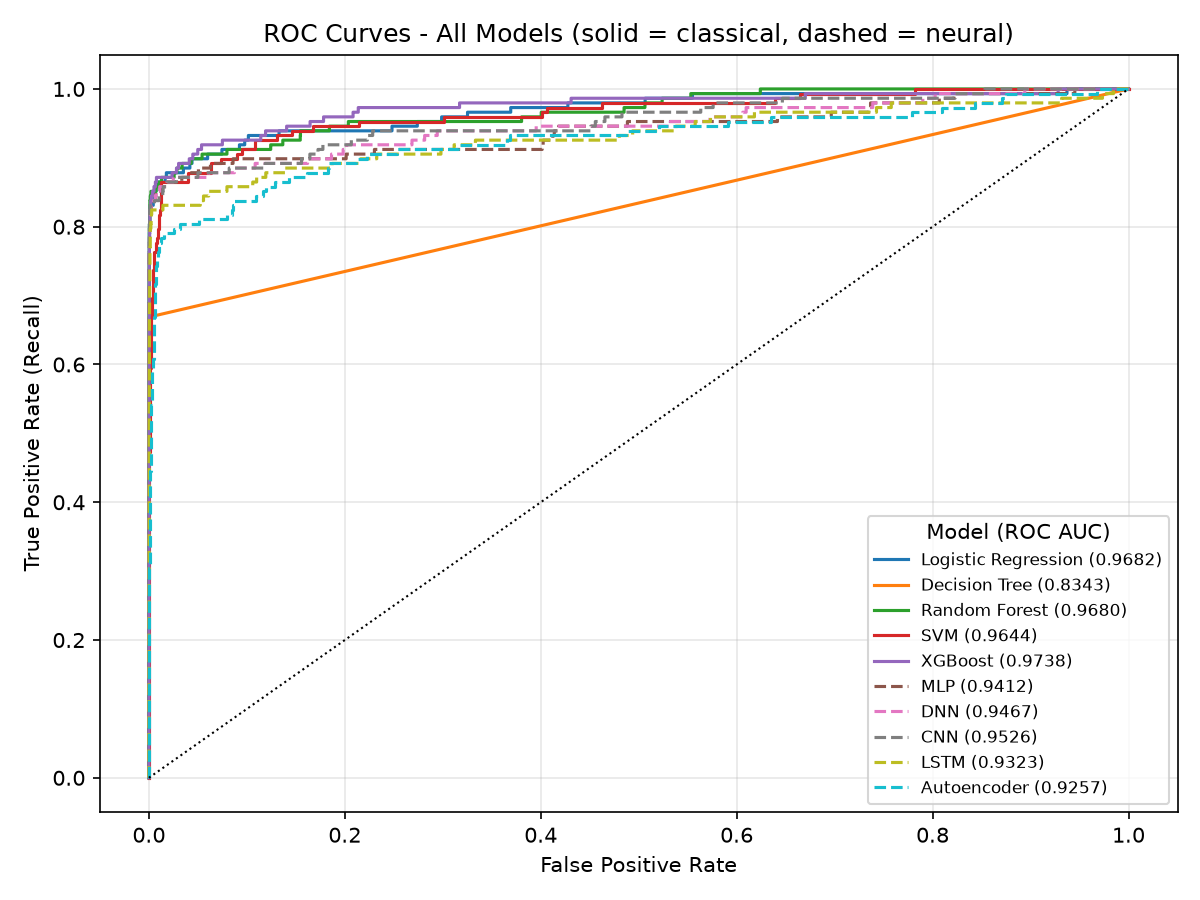
\includegraphics[width=\columnwidth]{roc_comparison.png}
\caption{ROC curves of all ten models (solid = classical, dashed = neural).}
\label{fig:rocall}
\end{figure}

\begin{figure*}[!t]
\centering
\newcommand{\roc}[1]{\includegraphics[width=0.19\textwidth]{roc_curves/#1.png}}
\roc{logistic_regression}\hfill\roc{decision_tree}\hfill\roc{random_forest}\hfill\roc{svm}\hfill\roc{xgboost}\\[2pt]
\roc{mlp}\hfill\roc{dnn}\hfill\roc{cnn}\hfill\roc{lstm}\hfill\roc{autoencoder}
\caption{Individual ROC curves. Top row, classical models: Logistic Regression (AUC = 0.9682), Decision Tree (0.8343), Random Forest (0.9680), SVM (0.9644), XGBoost (0.9738). Bottom row, neural networks: MLP (0.9412), DNN (0.9467), CNN (0.9526), LSTM (0.9323), Autoencoder (0.9257).}
\label{fig:rocgrid}
\end{figure*}

\textbf{Observations:}
\begin{itemize}
  \item XGBoost (AUC 0.9738), Logistic Regression (0.9682) and Random Forest (0.9680) have the strongest curves, rising steeply to about 85\% recall at a false positive rate close to zero.
  \item The neural networks' curves sit consistently below the classical ensembles, with AUCs between 0.9257 (Autoencoder) and 0.9526 (CNN).
  \item The Decision Tree's curve is a straight line through a single point, reflecting its near-binary outputs.
\end{itemize}
Confusion-matrix plots for every model are saved in \texttt{images/confusion\_matrices/}.

\section{Discussion}
\subsection{Performance Insights}
\begin{itemize}
  \item \textbf{Classical ensembles performed best.} XGBoost had the best ROC AUC and Random Forest the best F1 and PR AUC. Tree ensembles are well suited to tabular data like this, where each feature carries meaning independently and there is no spatial or sequential structure.
  \item \textbf{Neural networks did not outperform the classical models.} The MLP, DNN, CNN and LSTM reached similar recall but with roughly 3--6 times as many false alarms as XGBoost and 25--50 times as many as Random Forest. The CNN and LSTM architectures assume local or sequential structure that PCA-transformed features do not have, and the LSTM---the slowest model at 367.9 seconds---gained nothing from it.
  \item \textbf{The Autoencoder is useful when labels are missing.} Without any fraud labels it caught 80.4\% of fraud, though its false alarm rate makes it unsuitable as a stand-alone detector.
\end{itemize}

\subsection{Precision--Recall Trade-offs}
Class weighting tells every supervised model that missing one fraud costs as much as roughly 578 false alarms. At the default 0.5 threshold this pushes most models toward high recall and low precision, which is why Logistic Regression and all the neural networks flag over a thousand legitimate transactions each. The tree-based models were affected least: the Decision Tree and Random Forest raised fewer than 50 false alarms each, and XGBoost 415.

This shows that precision and recall at a single threshold depend as much on the weighting and threshold as on the model. The threshold-free metrics are a fairer comparison of the models themselves. Logistic Regression, for example, has a respectable PR AUC (0.7050) despite its 6.7\% precision at threshold 0.5, meaning a higher threshold would trade some recall for far fewer false alarms. In deployment, the threshold should be chosen on validation data to match the institution's cost of a missed fraud versus a false alarm.

\subsection{Classical ML vs.\ Neural Networks}
\begin{itemize}
  \item \textbf{Classical models} trained in 0.7--67.8 seconds (XGBoost: 2.3~s), need no validation set or early stopping, and offer better interpretability. On this dataset they also performed best.
  \item \textbf{Neural networks} took 55.9--367.9 seconds, required a separate validation set (leaving them 40\% of the data for training versus 70\% for the classical models), and were sensitive to class weighting and early stopping. Their strengths---learning from raw, high-dimensional, or sequential data---are not exercised by 30 pre-engineered PCA features.
\end{itemize}
Neural approaches would become more attractive with richer inputs, such as raw transaction histories per cardholder, where sequence models can learn behavioral patterns that tabular features cannot express.

\subsection{Interpretability Considerations}
\begin{itemize}
  \item \textbf{Logistic Regression} offers full transparency: each coefficient shows a feature's contribution to the fraud prediction, making it ideal for audits.
  \item \textbf{Tree ensembles} such as Random Forest and XGBoost provide feature-importance rankings and can be explained per prediction with tools such as SHAP, offering a practical middle ground.
  \item \textbf{Neural networks} such as CNNs and LSTMs are ``black boxes'' whose decisions require additional tools (e.g., SHAP, LIME) to explain.
\end{itemize}
Because the best-performing models here are also among the more explainable, this study found no trade-off between accuracy and interpretability on this dataset.

\section{Evaluation of Objectives}
\subsection{Objective 1: Compare Classical ML and Neural Networks on Real Fraud Data}
\textbf{Achieved.} Ten models---five classical and five neural---were implemented and evaluated on the same held-out test set, using both quantitative metrics and ROC curves.

\subsection{Objective 2: Preserve the Natural Class Distribution}
\textbf{Achieved.} No oversampling or undersampling was used. Imbalance was handled through class weighting, and the Autoencoder was trained only on legitimate transactions, in line with standard anomaly detection practice.

\subsection{Objective 3: Use Standard Evaluation Metrics}
\textbf{Achieved.} Every model was assessed with accuracy, precision, recall, F1-score, ROC AUC, and PR AUC, along with a confusion matrix and ROC curve.

\subsection{Objective 4: Address Interpretability vs.\ Predictive Power}
\textbf{Achieved.} The discussion contrasts interpretable models with black-box networks and finds that, on this dataset, the most accurate models are also reasonably explainable.

\subsection{Supporting Criteria}
\begin{itemize}
  \item \textbf{Consistency:} one shared pipeline, one shared test set, and training-only feature scaling for all models.
  \item \textbf{Reproducibility:} seeded randomness and a single command that regenerates every number and figure in this report.
  \item \textbf{Output coverage:} metrics, ROC curves and confusion matrices are saved for every model.
\end{itemize}

\section{Conclusion}
This study compared five classical machine learning models and five neural networks for credit card fraud detection, using a real, highly imbalanced dataset without any resampling and a single shared test set.

\subsection{Key Learnings}
\begin{itemize}
  \item Classical tree ensembles were the strongest models: XGBoost ranked fraud best (ROC AUC 0.9738) and Random Forest offered the best precision--recall balance (F1 0.7516, PR AUC 0.7975).
  \item Neural networks matched the classical models on recall but produced many more false alarms, ranked fraud less well, and cost far more to train. Sequence and convolutional architectures brought no benefit to tabular PCA features.
  \item The unsupervised Autoencoder caught 80.4\% of fraud with no labels at all, confirming its value for exploration or when labeled fraud is scarce.
  \item With imbalanced data, the class weighting and decision threshold strongly shape precision and recall, so threshold-free metrics (ROC AUC, PR AUC) are essential for comparing models fairly.
\end{itemize}

\subsection{Best Performing Models}
\begin{itemize}
  \item \textbf{XGBoost} (ROC AUC 0.9738, recall 85.1\%): the best ranking performance and the fastest of the ensembles to train.
  \item \textbf{Random Forest} (F1 0.7516, PR AUC 0.7975): the best operating point at the default threshold, with only 48 false alarms.
\end{itemize}

\subsection{Strengths and Limitations}
\begin{itemize}
  \item Evaluating on unmodified data, with one shared test set and training-only scaling, gives a realistic and fair comparison.
  \item Models used fixed, mostly default hyperparameters and a fixed 0.5 threshold. Systematic tuning, especially of class weights and thresholds for the neural networks, could change individual results.
  \item Results come from a single train/test split with 148 test frauds, so small differences between models (for example, a few frauds caught) are within normal variation. Repeated cross-validation would give confidence intervals.
  \item The PCA-anonymized features limit feature-level interpretation, and the two-day time span does not capture how fraud patterns change over time.
\end{itemize}

\subsection{Real-World Deployment Potential}
\begin{itemize}
  \item \textbf{XGBoost or Random Forest} suit real-time, explainable first-line detection, with the threshold tuned to the institution's cost of missed fraud versus false alarms.
  \item \textbf{An Autoencoder} can run alongside as a label-free second line, surfacing unusual transactions for review and helping detect new fraud patterns that supervised models have not been trained on.
\end{itemize}

\textbf{Final Thought:} More complex models are not automatically better. On structured tabular data, well-configured classical ensembles delivered the best detection, the lowest cost, and the most explainable decisions, while neural approaches are best reserved for richer data or for settings without labels.

\section{Supporting Literature and Relevance}
This project draws on prior work to ground its approach.

\textbf{Bhattacharyya et al. (2011)}~\cite{bhattacharyya} conducted one of the earliest large-scale comparisons of machine learning methods for credit card fraud detection, evaluating logistic regression, support vector machines, and random forests on real transaction data. They found that random forests performed best overall and that logistic regression remained competitive. This supports including classical baselines and is consistent with this study's finding that tree ensembles lead on tabular fraud data.

\textbf{Dal Pozzolo et al. (2018)}~\cite{dalpozzolo} argued that fraud detection systems must be evaluated under realistic conditions, accounting for the extreme class imbalance and for the limited number of alerts investigators can review. They recommend precision-focused measures over accuracy. This aligns with this project's decisions to keep the natural class distribution and to report precision, the number of false alarms, and PR AUC alongside ROC AUC.

By building on these works, this project extends the comparison to modern neural architectures and an unsupervised autoencoder, evaluated under the same realistic conditions.

\begin{thebibliography}{6}
\bibitem{bhattacharyya} S. Bhattacharyya, S. Jha, K. Tharakunnel, and J. C. Westland, ``Data mining for credit card fraud: A comparative study,'' \emph{Decision Support Systems}, vol.~50, no.~3, pp.~602--613, 2011, doi: 10.1016/j.dss.2010.08.008.
\bibitem{dalpozzolo} A. Dal Pozzolo, G. Boracchi, O. Caelen, C. Alippi, and G. Bontempi, ``Credit card fraud detection: A realistic modeling and a novel learning strategy,'' \emph{IEEE Trans. Neural Netw. Learn. Syst.}, vol.~29, no.~8, pp.~3784--3797, 2018, doi: 10.1109/TNNLS.2017.2736643.
\bibitem{kaggle} Machine Learning Group -- ULB, ``Credit Card Fraud Detection,'' Kaggle. [Online]. Available: \url{https://www.kaggle.com/datasets/mlg-ulb/creditcardfraud}
\bibitem{sklearn} scikit-learn User Guide. [Online]. Available: \url{https://scikit-learn.org/stable/user_guide.html}
\bibitem{xgboost} XGBoost Documentation. [Online]. Available: \url{https://xgboost.readthedocs.io/en/stable/}
\bibitem{keras} TensorFlow Keras Guide. [Online]. Available: \url{https://www.tensorflow.org/guide/keras}
\end{thebibliography}

\end{document}
